
\chapter{Decoupled Computational Pipeline as a Process Network}
\label{liveprof}
To facilitate the analysis of the pipeline of subgraphs generated from the original sequential program,
we relate it to a different model of computation, Kahn process network(KPN). which
provides the theoretical context for looking at issues such as deadlock and FIFO sizing in our pipeline. 


The KPN is an inherently
parallel model of computation where processes communicate with
each other through unbounded FIFO channels. 
The processes cannot test for availability of data tokens in 
the channels without consuming them. If a channel is empty
the process blocks as it reads from the channel.
Writing to the FIFOs, however, is non-blocking.
In addition, each FIFO can only be consumed by a single process, and be written to by a single process. The KPN model is deterministic in the sense that the scheduling of
the process execution does not alter the final results. This gives great flexibility
in implementing/controlling each individual processes. 
By relating our pipeline to KPN, or more precisely, observing its deviation from a pure
KPN, we can understand the freedom we have and the constraints we are subjected
to in our synthesis flow, where the correctness and liveness of the final implementation is required. Note the required absence of deadlock does not
apply to the eventual state of our pipeline, when the execution finishes.
As mentioned in section~\ref{sec:consp}, the execution of the pipeline completes when all subgraphs are either done running or waiting for inputs, which is a form of deadlock. This is expected and not the subject of our discussion in this
chapter.


%The generation of decoupled subgraphs from the original CDFG can actually be seen as a procedure which generates a more restricted version of KPN from sequential programs.
%As the shared global memory accesses do not fit into the KPN model naturally,
%we will have to first bridge this gap in their semantics(section~\ref{mp}). In implementing the network, we inevitably have to confront the boundedness of the
%FIFO channels, which may create deadlock situation depending on how each process
%are executed locally. We provide an analysis of the issue in  


\section{Memory and Fanout Process}
\label{mp}
A characteristic
of KPN is that all data exchange are performed over the FIFOs and the notion of
a shared global memory does not exist in the model. Previous works
converting sequential programs to process networks~\cite{mat2pn}\cite{c2stream}
were able to transform the original memory operations to explicit data IOs
at the boundary of the generated hardware as the targeted kernels are highly 
regular. In our case however, the synthesized pipelines may have irregular memory access patterns and are often used as accelerators along side a general purpose processor, the memory model needs to be preserved. It is therefore necessary to conceptually
translate the behavior of processes accessing memory to that of inter-process
communication.
%This is
%especially important as the generated accelerator is used in 
%conjunction with a general purpose processor which also shares
%the same memory subsystem. In another word, we need to 
%preserve the memory model in implementation but conceptualize
%the accesses in terms of distributed processes to allow for analysis.
%This is one area which was not addressed in previous works which 
%attempted to convert sequential programs to  process networks~\cite{mat2pn}\cite{c2stream}. They were targeting highly regular kernels where it is possible to
%have the original memory operations transformed to explicit data
%IOs at the boundary of the accelerator. In our case, however, the individual processes still access the shared memory directly, and we need to translate this behavior
%into that of communicating processes. 


In our system, the memory subsystem, including the associated interconnects, exposes multiple
input and output ports to the other hardware modules. 
Just like other processes in the network, through these ports, it consumes and produces tokens. In the case of load operations, addresses generated by the other processes
are read by the memory, and the corresponding data are returned. For store operations, on the other hand, the memory
consumes an extra data token while returning an acknowledge token.
This is certainly not sufficient to allow us to model it as
a conventional process in the network.
In particular, while a normal process blocks when reading from an empty
channel, the absence of requests at one input port never prevents the memory from serving requests from other ports. In another word, it can choose
which port to read depending on the availability of input tokens.
In YAPI~\cite{}, a ``select" function is added as an extension to the Kahn process network to support non-deterministic events. The behavior of
the shared memory subsystem can be accommodated with this primitive as well. 

With the introduction of ``select", the semantics of the original KPN is violated.
The memory subsystem can produce different output sequence depending on
the relative timing of appearance of token at its different input ports. 
This implies the scheduling of other processes would have an effect on the final
result of the execution, the system is no longer deterministic. 
However, as described in section~\ref{sec:partins}, we partitioned the memory
address space and added special memory-dependency edges between instructions. Consequently, the timing of memory requests coming from the normal processes are coordinated by the sending and receiving of special tokens among themselves.  This added constraint effectively eliminated any input token
sequences inconsistent with the behavior of the original sequential program,
while presenting the deviant memory ``process" a strict subset of the possible inputs. 
With the input streams across
different ports adhere to the read-after-write, write-after-read and write-after-write requirements encoded in the memory access instructions of the original program, the system becomes deterministic again. 

\begin{comment}
Thus we need 
to devise a mechanism such that only a certain subset of all possible input sequences
can ever be observed by the memory subsystem, and this subset would always result
in sequences of output tokens consistent with the behavior of the original sequential program.
%and this subset would always result
%in the same sequence of output tokens which is also consistent with the behavior of the %original sequential program. 
This is achieved by putting constraints on
the address/data streams generated by each process, which is in turn realized
by partitioning the address space and adding special memory-dependency edges between instructions, as mentioned in
chapter~\ref{sec:partins}. 
\end{comment}

\begin{figure}[htp]
\begin{center}

\includegraphics[width=0.85\linewidth]{chap4fig/memProcess.pdf}
\caption{Modeling Memory Access as Inter-process Communication
\label{fig:memproc}}
\end{center}
\end{figure}

In denotational semantics of KPN, each process is defined as a function mapping potentially infinite input streams to output streams, independent of the relative timing
of tokens in the streams.
After eliminating the possibility of the conventional
processes generating request sequences which violates memory dependency constraints, for all practical purposes, the memory subsystem can be seen as exactly that. 
%With 
%multiple input ports and multiple output ports however, 
%it cannot be described
%as a simple sequential process with blocking read, since the absence of requests at one port never prevents the memory from serving request from other ports. 
We can 
model it as a deviant process with no blocking read who, when scheduled, always takes a new request token and produces response/acknowledge token. This concept is visualized in figure~\ref{fig:memproc}. In particular, there is no sequential
ordering between the two response block $R1$ and $R2$, though within each block,
the operations are strictly ordered.






%we can see the memory subsystem as a process in the network whose
%output sequences do not depend on the scheduling of the network.  
%In denotational semantics of KPN, each process is defined as a function mapping %potentially infinite input streams to output streams. We can see the memory
%exactly as this mapping function when all the possible input streams across
%different ports adhere to the read-after-write, write-after-read and write-after-write requirements encoded in the memory access instructions of the original program. FIXME:adding picture for memory process 

%
%In the most trivial case, where each memory access operation in the original
%program is targeting a different part of the address space, the memory can
%be modeled as many little processes, each of which communicates with one memory %access
%operation in the process network, as shown in figure~\ref{}. This is however, an %unrealistic
%scenario, the memory is used for compute operations to communicate with each other
%temporally, therefore the accessed regions, more often than not, overlap with
%each other. 
%At the other end of the spectrum, we assume all the memory accesses
%are targeting the same memory location and all read-after-write, write-after-read
%and write-after-write ordering must be preserved, i.e. with a lot of memory-dependency-edges added in our CDFG. In this scenario, the memory
%can be modeled as one single process, who is only going to see
%the input sequences consistent with the order
%of memory accesses in the original program, and the sequences of tokens at each
%output port will be such that the actual 

%As mentioned in chapter~\ref{decoupleChap},  

%To model
%Given a specific input (token) history for a process, the process must be deterministic so that it always produces the same outputs (tokens)

%Given the partition of the memory address space, we can model each
%partition as 
%



Another requirement for KPN is the singularity of producers and consumers
for each channel. However, in a typical program represented in single static assignment form, value defined by an instruction can be used by multiple consumer instructions. 
To make it compatible with the KPN model, explicit fanout processes are added.
For every $1-to-n$ def-use relationship in the SSA, a fanout process with one
input and $n$ outputs is added. The process duplicates every input token $n$ times and sends one to each of the consumer processes. 
As shown in figure~\ref{fig:fanout}, a
fanout process, just like other processes created from partitioning CDFGs, consists
of a sequence of instructions, some of which consume tokens while others produce and transmit tokens. 
With the addition of these processes all the channels in the network are one to one and we have a conceptualization of the entire computation described by the original program
in terms of a KPN, with the addition of a more flexible memory ``process''.

\begin{figure}[htp]
\begin{center}
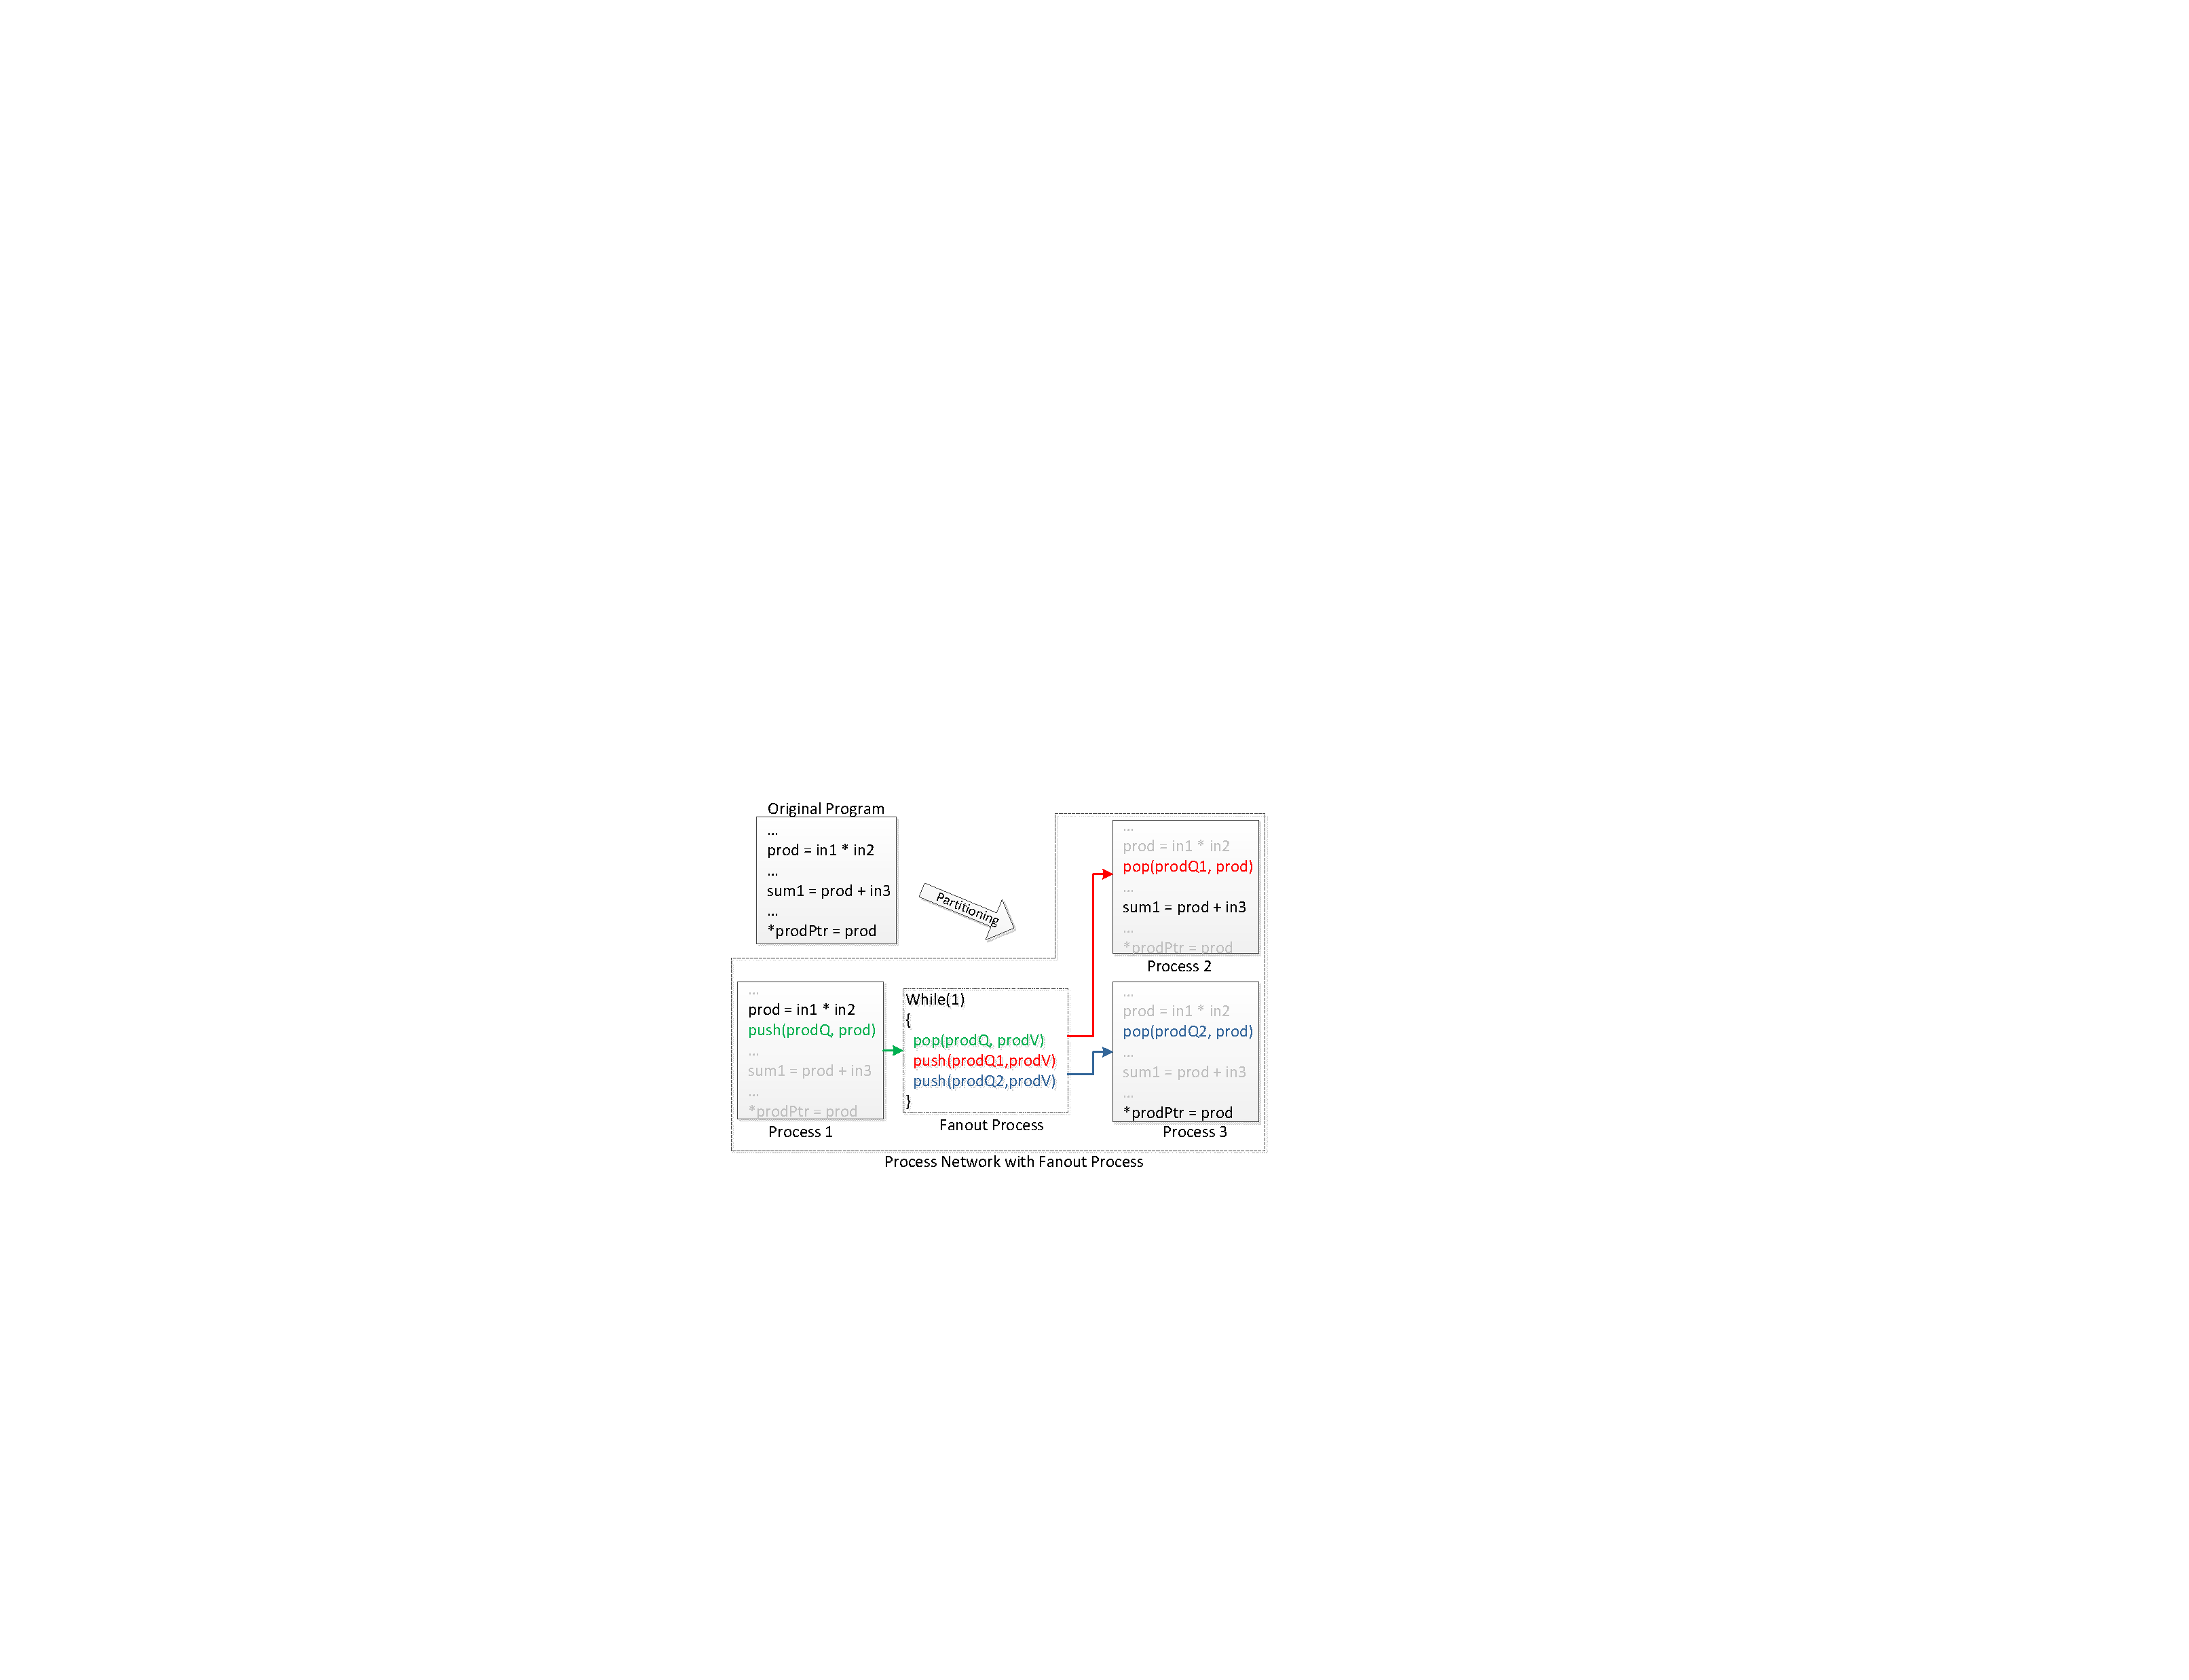
\includegraphics[width=0.65\linewidth]{chap4fig/fanout.pdf}
\caption{Addition of Fanout Process while Partitioning
\label{fig:fanout}}
\end{center}
\end{figure}



\section{Bounded Execution of the Process Network}
In real implementation of a KPN, 
it is impossible to have unbounded communication FIFOs between
processes. In~\cite{}, KPNs are 
categorized into strictly bounded, bounded and unbounded ones.
A KPN is strictly bounded if and only if any execution of of the network requires bounded space. It is bounded if and only if there are some
execution requiring bounded space while it is unbounded if and only if any
execution requires unbounded space. Methods to find bounds for communication channels
in KPNs were discussed in~\cite{}\cite{}. In general, whether a
KPN is bounded is undecidable~\cite{}, but for our process networks, which
are generated from sequential programs expressed in single static assignment
form, we can analyze the boundedness of the FIFO channels in various
scenarios. Note here we try to deduce properties applicable for
networks created by any arbitrary partitioning algorithms applied to
the original CDFG. Thus they also apply to the pipeline generated
using method outlined in chapter~\ref{decoupleChap}, which is just
one specific instance of all possible KPNs producible from a sequential program.


More specifically, given a sequential program $S$ in single static assignment form, we can partition the program into a process network $N$, consisted of a set of normal processes $P$, a set of fanout processes $F$, and a memory process $M$. 
Also, as mentioned in chapter~\ref{decoupleChap}, if an instruction is assigned to
$p$ and it is taking in tokens from instructions in other processes, a placeholder
instruction (and its owner basic block) is instantiated local to $p$, whose sole purpose is to receive
the actual token from the producer/fanout process. For $M$, it can be seen as containing a mirroring of all the memory accessing
instructions distributed among $P$, and each of its mirrored instructions 
produces tokens for the corresponding $p$ to consume.

\begin{definition}
Let $I$ be the set of instructions in the original $S$. For every $i \in I$, each
execution of $i$ is defined as a instruction instance $i_k$, where $k \in \Bbb{Z}$.
 In each $p \in P$, 
every instruction $j \in J^p$ corresponds to one $i$ in $S$, and every execution of this instruction $j_k$ corresponds to one $i_k$ in $S$. Let 
each of the placeholder/consumer instructions in $p$ be $\underline{j}$, and each instruction actually producing value to transmit be $\overline{j}$, every instance
of $\underline{j}$/$\overline{j}$ in the same process reads from/writes to the same FIFO channel. Note for each $\overline{j} \in J^p$,
there will be one or more  $\underline{j} \in J^{p'}$ where $p' \in P\setminus p$, and they are connected either directly or through $f_i \in F$. Also let the set of $\overline{j}$
 and $\underline{j}$ in $p$ be $\overline{J^p}$ and $\underline{J}^p$ respectively,
 we then have $\overline{J^p} \cup \underline{J}^p \subseteq J^p$ as some instructions may be strictly used locally.
\end{definition}



\begin{lemma}
\label{bounded}
Any instance of network $N$ is bounded with FIFO space required for each channel = 1.
\end{lemma}




To prove Lemma~\ref{bounded}, we can constructively create an execution schedule $H$
which does not overflow the FIFOs of size 1. This can be performed by following the original program order in $S$. 
Whenever a instruction instance $i_k$  of $i$ is executed in $S$, we find its corresponding set in $P$, these are instructions distributed among one or more processes.
For each element $j \in J^p, p \in P$ in this set:
\begin{itemize}
    \item If $j \not\in \overline{J^p} \cup \underline{J}^p$, we can just schedule $j_k$.
    \item If $j \in \overline{J^p}$, i.e. it is a ``producer" instruction, $j_k$ is scheduled and then the instructions in $f_i$ are scheduled (assuming there is fanout), followed by all the other ``consumer" instructions $j' \in \underline{J}^p', p' \in P\setminus p$.
    

%If $i_k^p \in \overline{I^p}$, the fanout process $f_i$, if there is any, is then scheduled. Subsequently, all the $\widetilde{i_k^p'}$ are scheduled.
    \item If $j_k$ accesses memory, then the instructions in the corresponding response block in $M$ is immediately scheduled to serve the request before everything else.
    \item If $j \in \underline{J}^p$, do not schedule it directly, wait for the producer instruction and $f_i$ to be scheduled.
\end{itemize}
Since the consumers of the tokens are always executed immediately after the producer instruction, the FIFOs will not see a backlog of tokens.

\begin{definition}
Let the schedule of instructions in each $p \in P \cup F$ be $G(p)$, we say $G(p)$ is locally consistent with $H$ if
and only if
$j'_x \prec j''_y$ in $H$ $\Rightarrow$ $j'_x \prec j''_y$ in $G(p)$
, $\forall j', j'' \in J^p$, 
$x, y \in \Bbb{Z}$. Additionally, if we have a schedule $H_s$ for a set of instruction instances  which can belong to different processes, we say $H_s$ is globally consistent with
$H$ if and only if $j'_x \prec j''_y$ in $H$ $\Rightarrow$ $j'_x \prec j''_y$ in $H_s$
 where  $x,y \in \Bbb{Z}, j' \in J^{p1}, j'' \in J^{p2}, p1 \in P \cup F, p2 \in P \cup F$.
\end{definition}


It should be apparent that if instances of a producer/consumer
instruction pair around a FIFO are globally consistent to $H$, we
do not need to have FIFOs with size greater one for our execution.
Meanwhile, as $H$ is derived from the original program order of
the sequential program $S$, all locally consistent schedules $G(p)$ 
do not violate data dependencies imposed by $S$.


\section{Artificial Deadlock in Process Network}
In actual implementation of KPN where FIFOs have fixed sizes, blocking
writes are introduced so that processes block when trying to write to a full FIFO.
This induces artificial deadlock as described in~\cite{}. 
When an artificial deadlock occurs, a circular dependency is formed among
processes, none of whom can make progress. At least one of the processes
in the cycle is blocked on write -- therefore the deadlock is ``artificially''
introduced by the size limit of FIFOs. 

Being a network of sequential processes and memory connected together by
bounded FIFOs, the computational pipeline synthesized may experience
artificial deadlocks as well. The interaction between the sizing of the FIFOs 
and the occurrence of deadlocks needs to be analyzed to ensure the liveness
of our pipeline.
\begin{comment}
\begin{lemma}
\label{blockingwriteconsistent}
In the presence of blocking writes, given a pair of instruction $\overline{j'} \in p1, \underline{j}'' \in p2$ writing to and reading from a FIFO, all their
instances are globally consistent with $H$ if the FIFO is of size one.
\end{lemma}

Lemma~\ref{blockingwriteconsistent} can be proven by contradiction.....
\end{comment}
\begin{lemma}
\label{nondeadlock}
Assuming requests to $M$ is first-come first-served,
all FIFOs are of size one and blocking write,
as long as $G(p), \forall p \in P \cup F$ are locally consistent with $H$,
artificial deadlock will not occur in $N$. 
\end{lemma}

Assume there is an artificial deadlock, we can go around the dependency
cycle and examine the blocked processes $P_b \subseteq P \cup F$. For a process $p_b$
to be blocked at instruction instance $j_k$, $j_k \in J^p$ is either reading from an empty
FIFO, or writing to a full FIFO. For the former case, the FIFO is empty because the producer of the token
$j'_k \in J^{p'}$ cannot execute, which indicates an earlier instruction 
instance $l_m$ in $G(p')$ is blocked. For the later case, the FIFO is full because the consumer $j''_{k-1} \in J^{p''}$ of the earlier token produced by
$j_{k-1}$ cannot execute, which also indicates an earlier instruction in $G(p'')$
is blocked. Apply this reasoning recursively around the circle of dependencies,
we have a chain of instructions instances $j_k \succ l_m \succ ... \succ j_k$
or $j_k \succ j''_{k-1} \succ ... \succ j_k$ in $H$, as each pair in the chain
comes from a schedule locally consistent with $H$. This chain is self-contradictory
and therefore the scenario for artificial deadlock can never occur. 

The memory subsystem, being FCFS, always produces tokens some processes are waiting to consume, there is no possibility of it being blocked on write, and thus being
part of the dependency cycle causing the deadlock.


As each $G(p), p \in P \cup F$ is locally consistent with $H$, which is derived from
the program order of the original $S$, we can conclude that if each of
the generated subgraph is executed strictly according to the original
program order, we will have a pipeline free from artificial deadlock. This
will guarantee, for instance, when processors are used as the execution substrate, the network will produce the correct result as
each process is executed according to program order. On the other hand, when
HLS is used to create hardware accelerators from them, this guarantee may not
hold anymore since aggressive parallelization and reordering of instructions
would violate the consistency between $G(p)$ and $S$. We thus need to examine
the  effect of instruction reordering on the liveness of our pipeline.



\begin{figure}[htp]
\begin{center}
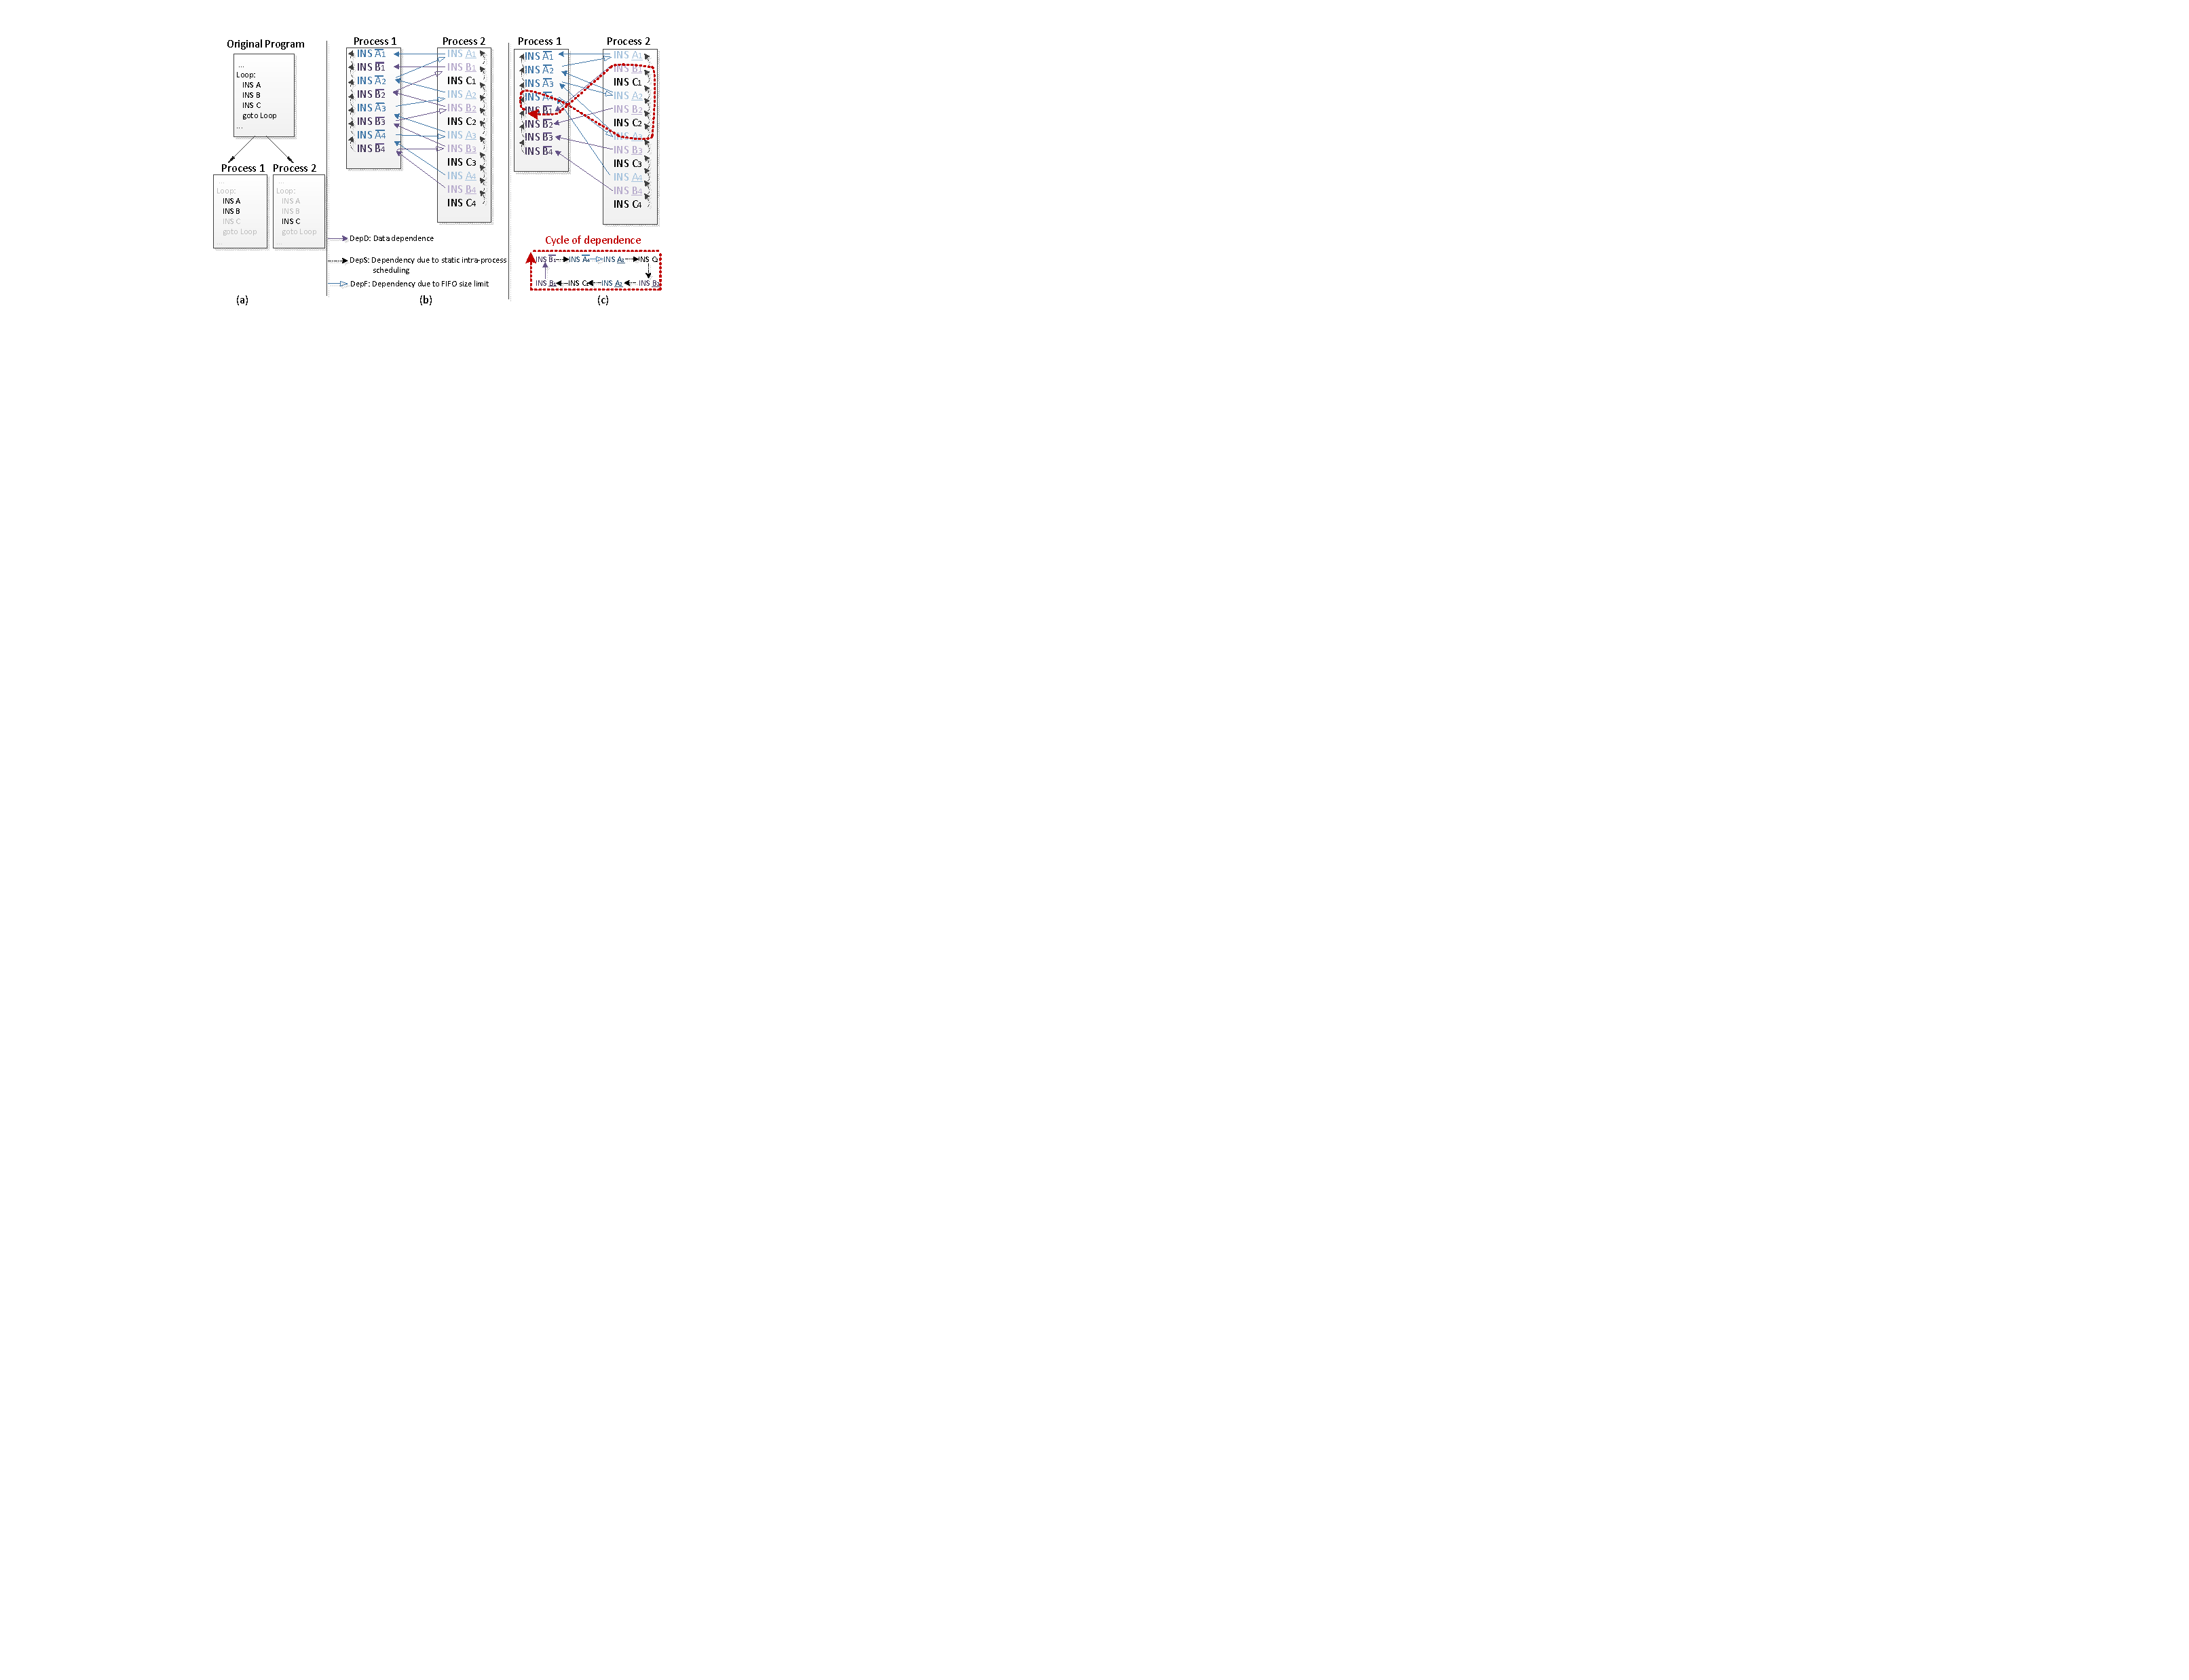
\includegraphics[width=1.0\linewidth]{chap4fig/cycleInstances.pdf}
\caption{a) partitioning of the original program into two processes; b) each process executes according to the program order; c) instructions in process 1 are reordered statically
\label{fig:deadlockfig}}
\end{center}
\end{figure}

\section{Liveness in HLS-generated Computational Pipeline }
Figure~\ref{fig:deadlockfig} shows a simple example of a otherwise deadlock free network becomes problematic
when the instructions are statically reordered in individual processes by HLS. 
Due to the size limit of the FIFOs, which is assumed to be one here, the execution
of the producer instruction is dependent on the completion of the previous instance
of the consumer instruction. In figure~\ref{fig:deadlockfig}(c), when the instructions in process 1 is statically reordered, a circular dependency is formed
between instructions: INS $\overline{B_1}$ cannot execute unless
INS $\overline{A_4}$ completes, and INS $\overline{A_4}$ cannot execute until
INS $\underline{A_3}$ consumes the token from INS $\overline{A_3}$. But INS $\underline{A_3}$ cannot happen until INS $\underline{B_1}$ occurs, and
that depends on the completion of INS $\overline{B_1}$.  An artificial deadlock
is therefore created. 

In this particular example, if the size of FIFO for $\text{INS }A$ is increased
from 1 to 3, then the execution of INS $\overline{A_4}$ would be dependent on 
INS $\underline{A_1}$ instead of INS $\underline{A_3}$. The
channel can now buffer the tokens produced by INS $\overline{A_1}$ -- INS $\overline{A_3}$ before INS $\underline{A_1}$ needs to be invoked to create empty slot. With this increase in buffer space, the cycle of dependence is broken as there will be no path of dependence from INS $\underline{A_1}$
to INS $\overline{B_1}$. The deadlock no longer exists.


Indeed, this is the classic approach in resolving artificial deadlock~\cite{}. 
When artificial deadlock is detected, the process which is write blocked is found, the full FIFO it tries to write to is given more capacity. 
However, in a network implemented in hardware, the FIFO size cannot be easily increased.
%As the producer and consumer instruction instances are rescheduled differently with
%respect to other instructions in their own process, blocking write causes
%artificial deadlock. Increasing the number of slots in the FIFO can help resolve
%this problem. 
To determine the needed buffer space in the channels \textit{a priori}, simulations are sometimes used~\cite{}. It relies 
on using representative dataset as input and for certain type of problems, simulation results may not provide any guarantee, especially if the control flow is runtime data dependent. In this section, we want to analyze the interaction between FIFO
sizing and intra-process instruction scheduling, 
so we can better understand
their joint effect on the liveness of the process network. 
%what kind of reordering can be permitted and its effect on the FIFO space needed.
\begin{comment}
We have proven that when each $p \in P$ execute according to the original
problem order, no artificial deadlock would occur even when the FIFO is of size one.
Our example shows that when producer (or consumer) instructions are rescheduled with respect to other instructions in their own process, more tokens may
need to be buffered before the consumer instruction is activated. To ensure progress
of the network, we need to size the FIFOs such that a
consumer instruction instance is always scheduled before the cycle of blocked
processes is formed.
\end{comment}
\subsection{Artificial Deadlock Detection without Simulation}
In our networks derived from sequential programs, given each process' schedule and each FIFO's size, it is possible
to find out if a potential artificial deadlock can arise without running simulation. As demonstrated in figure~\ref{fig:deadlockfig}, we can add $DepS$ edges between instruction instances belonging to the same process, and $DepF$ edges between
producer/consumer instruction instances writing/reading from the same FIFO.
Note for a FIFO of size $s$, $DepF$ edges are added between $\overline{j_k}$ and $\underline{j_{k-s}}$ to indicate that the producer instruction instance is disabled
until the consumer instruction instance is invoked. The graph thus obtained
can be checked for cycles, which indicate the occurrence of artificial deadlock.


The schedule for each process may contain potentially infinite instruction instances, resulting in a graph with infinite number of nodes,
which makes it impossible to guarantee the absence of artificial deadlock.
However, when we use HLS tool to map each process,
a short, repeatable schedule is generated and we can represent the
dependencies between instruction instances using a manageable
sized graph. 
%Meanwhile, we
%can take advantage of the transitive property of dependencies 
%to reduce the number of edges in the graph as well. 
Figure~\ref{fig:singlelevelLoopCylce} shows a more concise
representation of the schedule we have in figure~\ref{fig:deadlockfig}(c).
Various dependency edges are associated with weights to 
represent the difference between the subscripts of the pair of instruction
instances. For instance, as INS $\overline{A_4}$ is 
scheduled before INS $\overline{B_1}$ in process 1, the edge from INS $\overline{B}$ to INS $\overline{A}$ carries
a weight of 3, meaning the occurrence of INS $\overline{B_x}$ depends on the completion of INS $\overline{A_{x+3}}$. Similarly, when the channel between 
INS $\overline{A}$ in process 1 and INS $\underline{A}$ in process 2 are of size one, INS $\overline{A_x}$ depends on the completion of INS $\underline{A_{x-1}}$, 
which is represented by the $-1$ weight of the edge representing this
dependency. The edges denoting data dependencies between processes
are always of weight 0, as each pair of the end points represents the same instruction instance, with one being the actual source of the data, and the other a placeholder in the consumer process.
Note the weights assigned correspond to the largest differences
in instance subscripts, representing the furthest an instruction is running
ahead of its dependents. In the presence of branches, it is possible that
an instruction does not get executed every loop iteration. The subscripts
assumed by the instruction instances do not take this into account, i.e. $I_3$
in iteration 3 despite it is actually the second time $I$ is executed. Thus under
this particular scheme, the subscripts assigned to instruction instances
are just the iteration numbers of the enclosing loop in the original program.
Note in the literature about loop dependency analysis~\cite{Kennedy:2001:OCM:502981}, the term iteration number is generally associated with analyzable loop index, with
bounds and regular change steps. Here, however, we just use the term to represent the simple ordering of iterations, with or without actual loop indices.

To shrink the size of the graph, we have taken advantage of the transitive property of dependencies to reduce the number of the $DepS$ edges in the graph.
As only the scheduling of producer/consumer instructions matters for
deadlock detection, we can further trim the graph by omitting any $DepS$ edges having end point $j \not\in \bar{J^p} \cup \underline{J}^p$. In figure~\ref{fig:singlelevelLoopCylce}, for instance, the $DepS$ from INS $\underline{A}$ to INS $C$ can be redirected to INS $\underline{B}$, accompanied by the deletion of INS $C$ and the $DepS$ edge from INS $C$ to INS $\underline{B}$.


\begin{figure}[htp]
\begin{center}
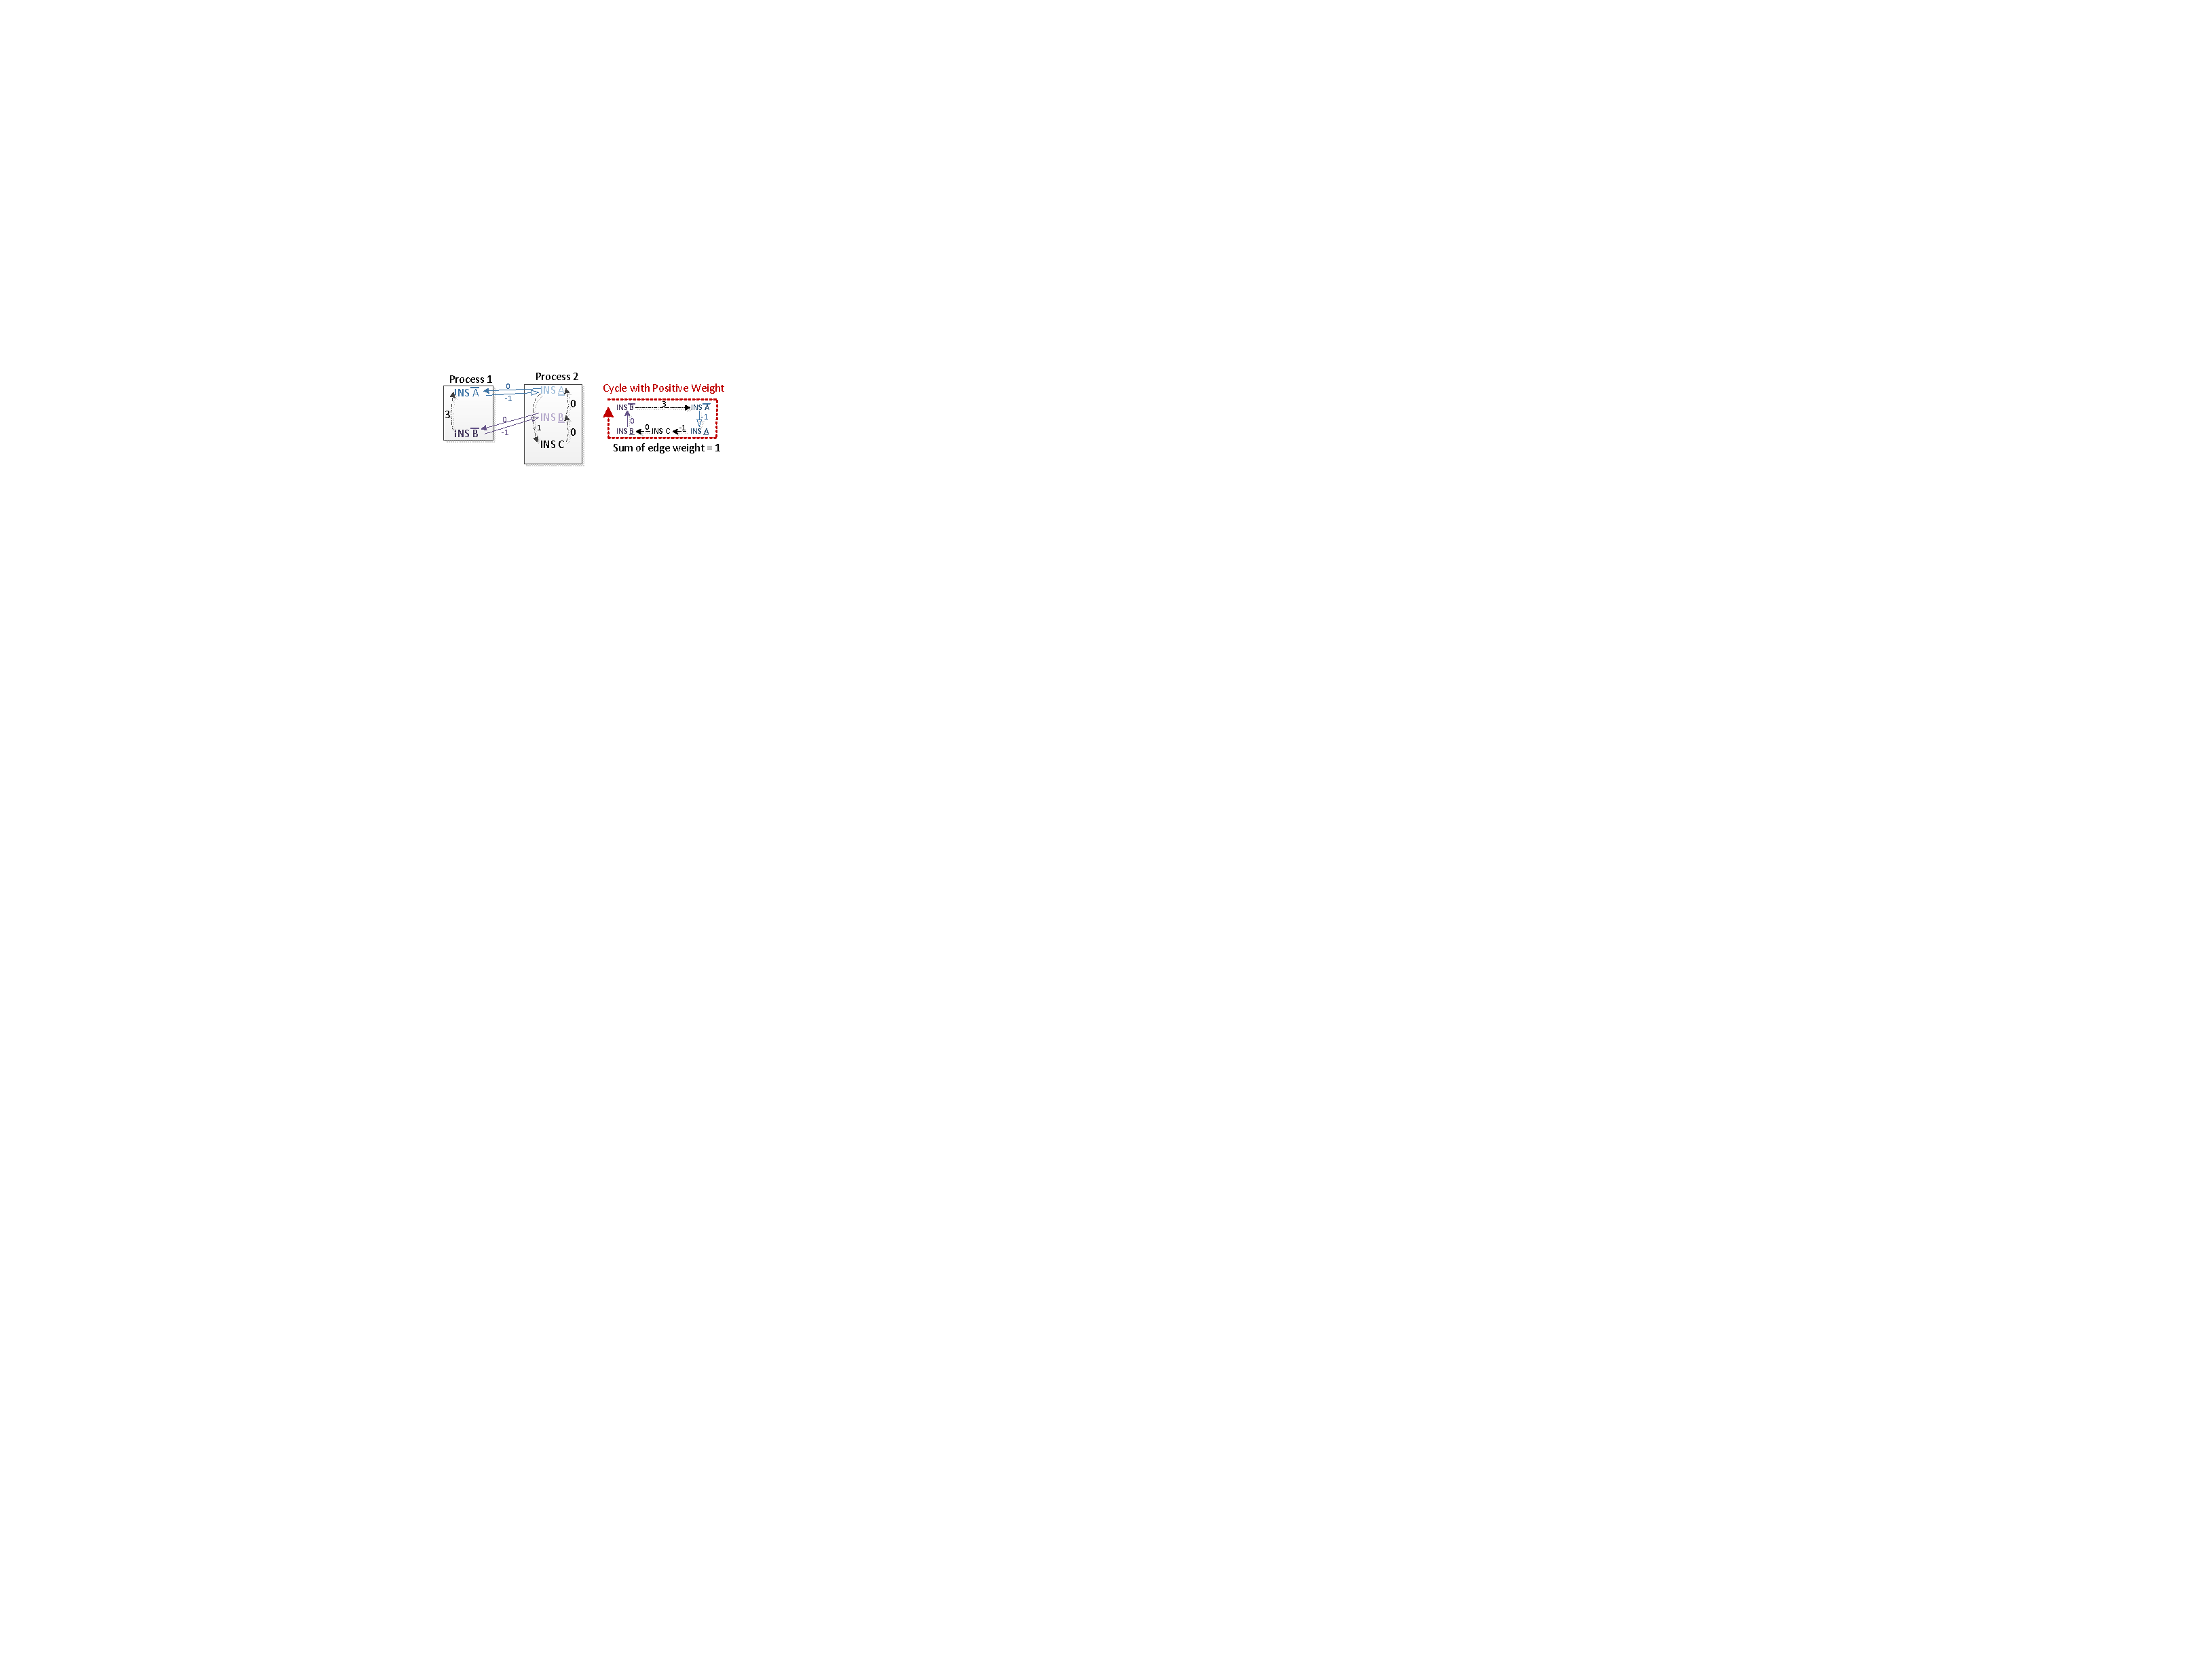
\includegraphics[width=0.7\linewidth]{chap4fig/singlelevelLoopCycle.pdf}
\caption{Deadlock Detection using Graph with Weighted Edge
\label{fig:singlelevelLoopCylce}}
\end{center}
\end{figure}

Now, if a non-negatively weighted cycle is found within this graph, we have an artificial deadlock.
A cycle in the graph means we have an instruction instance $I_x$, whose occurrence depends on the completion of $I_{x+w}$, $w$ being the weight of the cycle.
With $w$ being greater or equal to zero, $I_x$ cannot happen until itself or a later instance happens -- we have a deadlock. 
The computation to find deadlocks may potentially be expensive. In the worst case, the number
of simple cycles in the graph can be exponential in
$|V|$, the number of nodes in the graph. Practically however, the number of
nodes involved are approximately the same as the number of channels needed, while the graph is rather sparse in the connectivity between these nodes. 
Methods such as~\cite{doi:10.1137/0204007} can be used for efficient
enumeration of the cycles and the subsequent identification of the deadlocks.



Resolving
the deadlock involves choosing one of the $DepF$ edges
in the cycle and add enough slots (making the weight more negative)
such that the sum of the edge weights becomes negative. For
one particular cycle, the $DepF$ edge whose channel has the smallest width can be selected, as this minimizes the cost of adding the extra slots. However,
as multiple non-negatively weighted cycles can be present simultaneously,
the global optimal solution would involve finding a set of $DepF$ edges, 
and minimize the aggregate cost of incrementing each for all cycles to be resolved, which 
is NP-Hard. (maybe I shall formulate an ILP here??)
\begin{figure}[htp]
\begin{center}
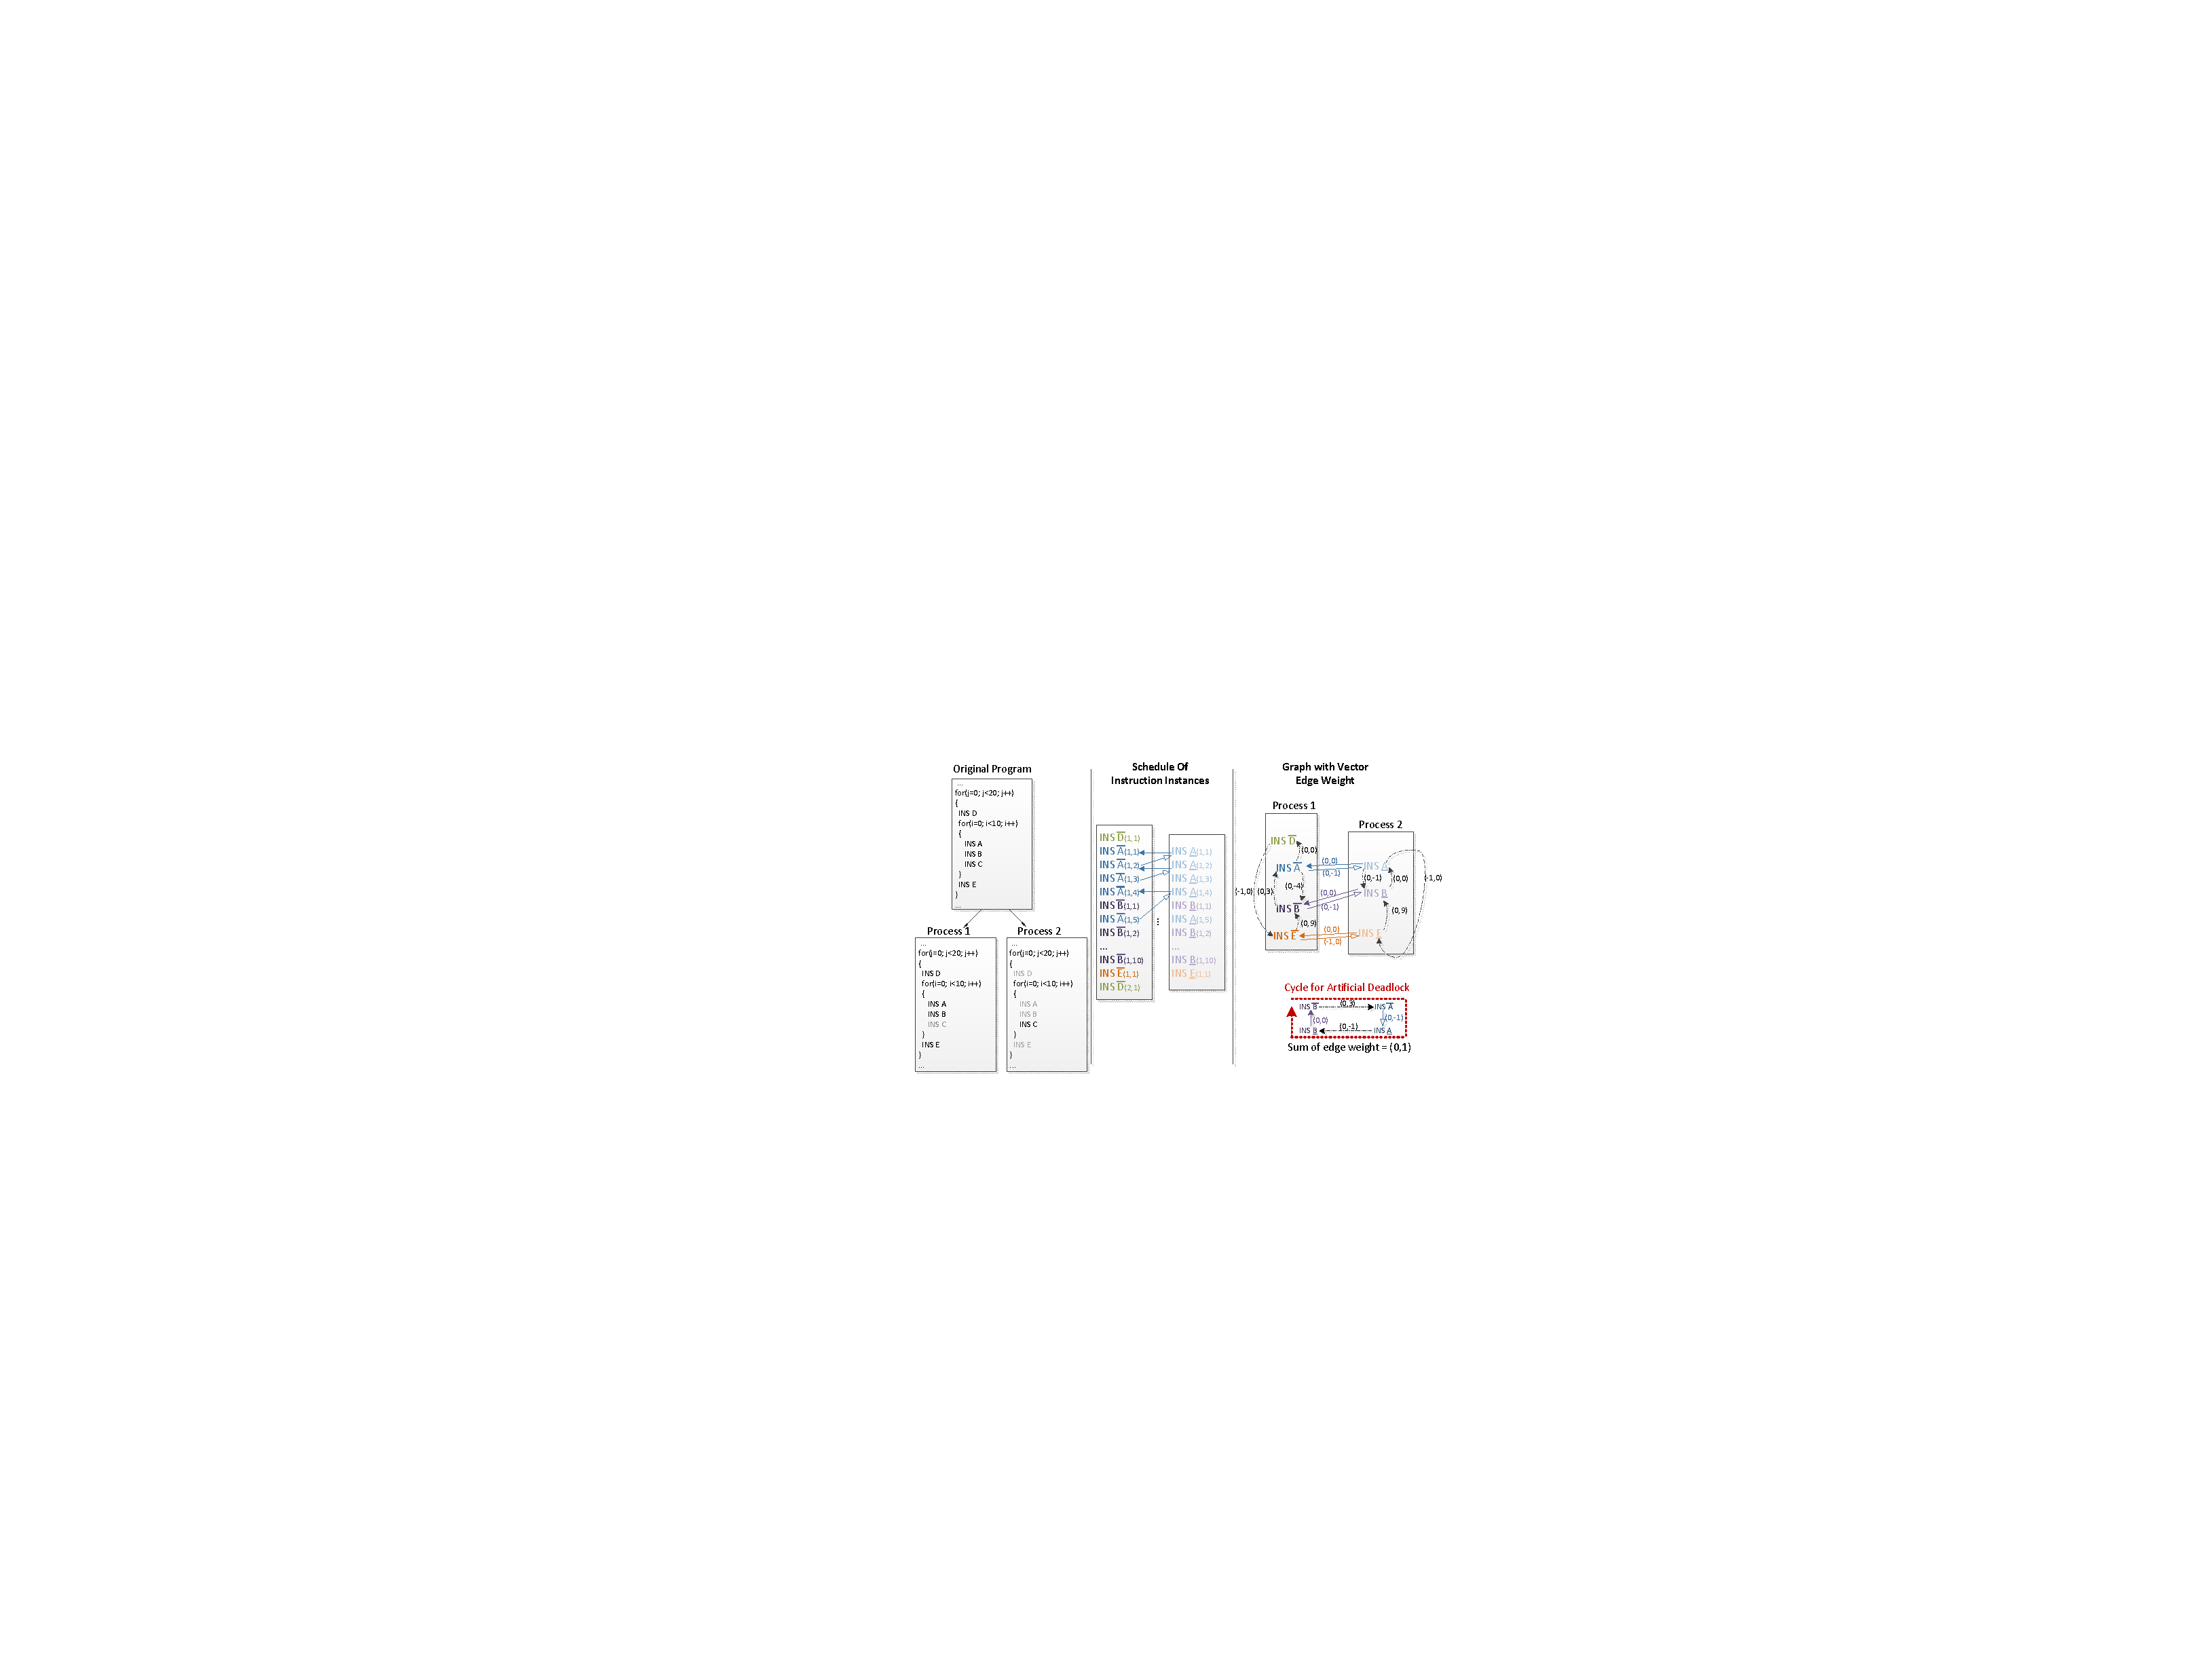
\includegraphics[width=1.0\linewidth]{chap4fig/vectorAnnot.pdf}
\caption{Multi-level Loop Nest Deadlock Detection
\label{fig:vectorannot}}
\end{center}
\end{figure}

So far we have formulated a method for deadlock detection and resolution
for a single level loop. To generalize this method for loop nests of multiple
levels, we associate each instruction instance with
a vector of iteration numbers, with the earlier elements corresponding to the outer loops.
%indicating its position in the iteration space.
Subsequently, for the weight assigned to each of the edges, instead of
a single number, a vector is used. The number of elements in the vector
corresponds to the number of levels in the loop nest.
An example of this is shown in figure~\ref{fig:vectorannot}. 



All the vector weights assigned to the edges between instructions of
the same level in the loop nest are really the same as in the single level loop
example, except the padding of zeros to match the dimension of the iteration space. A more interesting case is the $DepS$ edge from INS $\overline{E}$ to INS $\overline{B}$, which goes from an outer loop instruction to an inner loop instruction. 
The last components of the subscript vectors of INS $\overline{E}$ instances are always 1
as the instruction does not execute in the innermost loop. The subscript vectors of INS $\overline{B}$ instances, however, can take a value up to 10 for its right most element, as the inner most loop has an iteration count of 10. Thus the weight $(0,9)$
means the $1$st INS $\overline{E}$ instance is scheduled after the $10$th occurrence of INS $\overline{B}$ in the current iteration of the outer loop.

In this modified graph, 
every cycles in the graph now has a weight sum which is also a vector. 
An deadlock is manifested as a cycle with weight being the zero vector ($\vec{0}$)
or vectors whose first non-zero elements (leading elements) are positive.
Similar to the case when we have scalar
weights, these weight vectors 
indicate an instruction instance depending on itself or a later instance in the iteration space, and thus a deadlock. The deadlocks can also be
resolved by finding the $DepF$ edges, whose change of capacity makes
all the cycles' weights' to have negative  leading element. 


\begin{definition}
When an artificial deadlock occurs, a cycle of dependency between instruction instances is formed. Define this cycle as $C_v$. Each instruction instance in $C_v$ corresponds to one instruction in the weighted graph. Define the cycle formed in the weighted graph by the corresponding instructions as $C_V$, and the set of instructions
as $V$. 
\end{definition}

As mentioned before, non-communicating instructions/instruction instances can be omitted in the graph without affecting the deadlock analysis, thus $V \subseteq \bar{J^p} \cup \underline{J}^p$. As the nodes in $C_v$ are instantiations of nodes in $C_V$, the edges in $C_v$ are also
instantiations of edges in $C_V$. Let these edges in $C_v$ carry the same weights as the $C_V$ edges they instantiate.

\begin{lemma}
\label{deadlock2cycle}
If there is an artificial deadlock in the network, there will be a cycle in
the weighted graph whose sum of edges
is either $\vec{0}$ or vectors with positive leading element. 
\end{lemma}

% we wanna prove the sum of edges in C_i is smaller than C_I
%Assume $C_I$'s weight has negative left most non-zero element, 
We can take any point in  $C_v$, and go around the
cycle $C_v$ to get a sequence $V^1_{X1}$, $V^2_{X2}$ ... $V^n_{Xn}$ where $V^1 ... V^n \in V$, $V^1 = V^n$ and $X_1 = X_n = X_1 + (X_2-X_1) + (X_3-X_2) ... (X_n - X_{n-1})$. The sum of edges in $C_v$ = $(X_2-X_1) + (X_3-X_2) ... (X_n - X_{n-1})$ =$\vec{0}$ as $X_1 = X_n$.  

If no two elements in $C_v$ map to the same
element in $V$, then the sum of edges in $C_v$ is equivalent to the 
sum of edges in $C_V$, which would be zero -- we have a cycle in the weighted
graph whose sum of edges is the $\vec{0}$.

Otherwise, we can have $C_v$ containing two instruction instances $U_{Y1}, U_{Y2}$ mapping to the same element $U \in V$, and instruction instances on the path between $U_{Y1}, U_{Y2}$ are all unique instances of instructions in  $W_1 \subseteq  V \setminus U$.  
Now we can construct a cycle $C_{W1}$ of instructions using $W_1$, and the weight of this cycle is the same as the weight of the path from $U_{Y1}$ and 
$U_{Y2}$ as every edge in the path is a unique instantiations of a corresponding edge in $C_{W1}$. This decomposition can be applied recursively to 
the remaining part of $C_v$ until we have $C_{W1}, C_{W2}...C_{Wn}$ whose
sum equals to the weight of $C_v$. Since weight of $C_v$ is  $\vec{0}$, 
they can either all be of weight $\vec{0}$, or at least one of them will have
positive leading element. This process is illustrated in figure~\ref{fig:decomp} for a single level loop.

\begin{figure}[htp]
\begin{center}
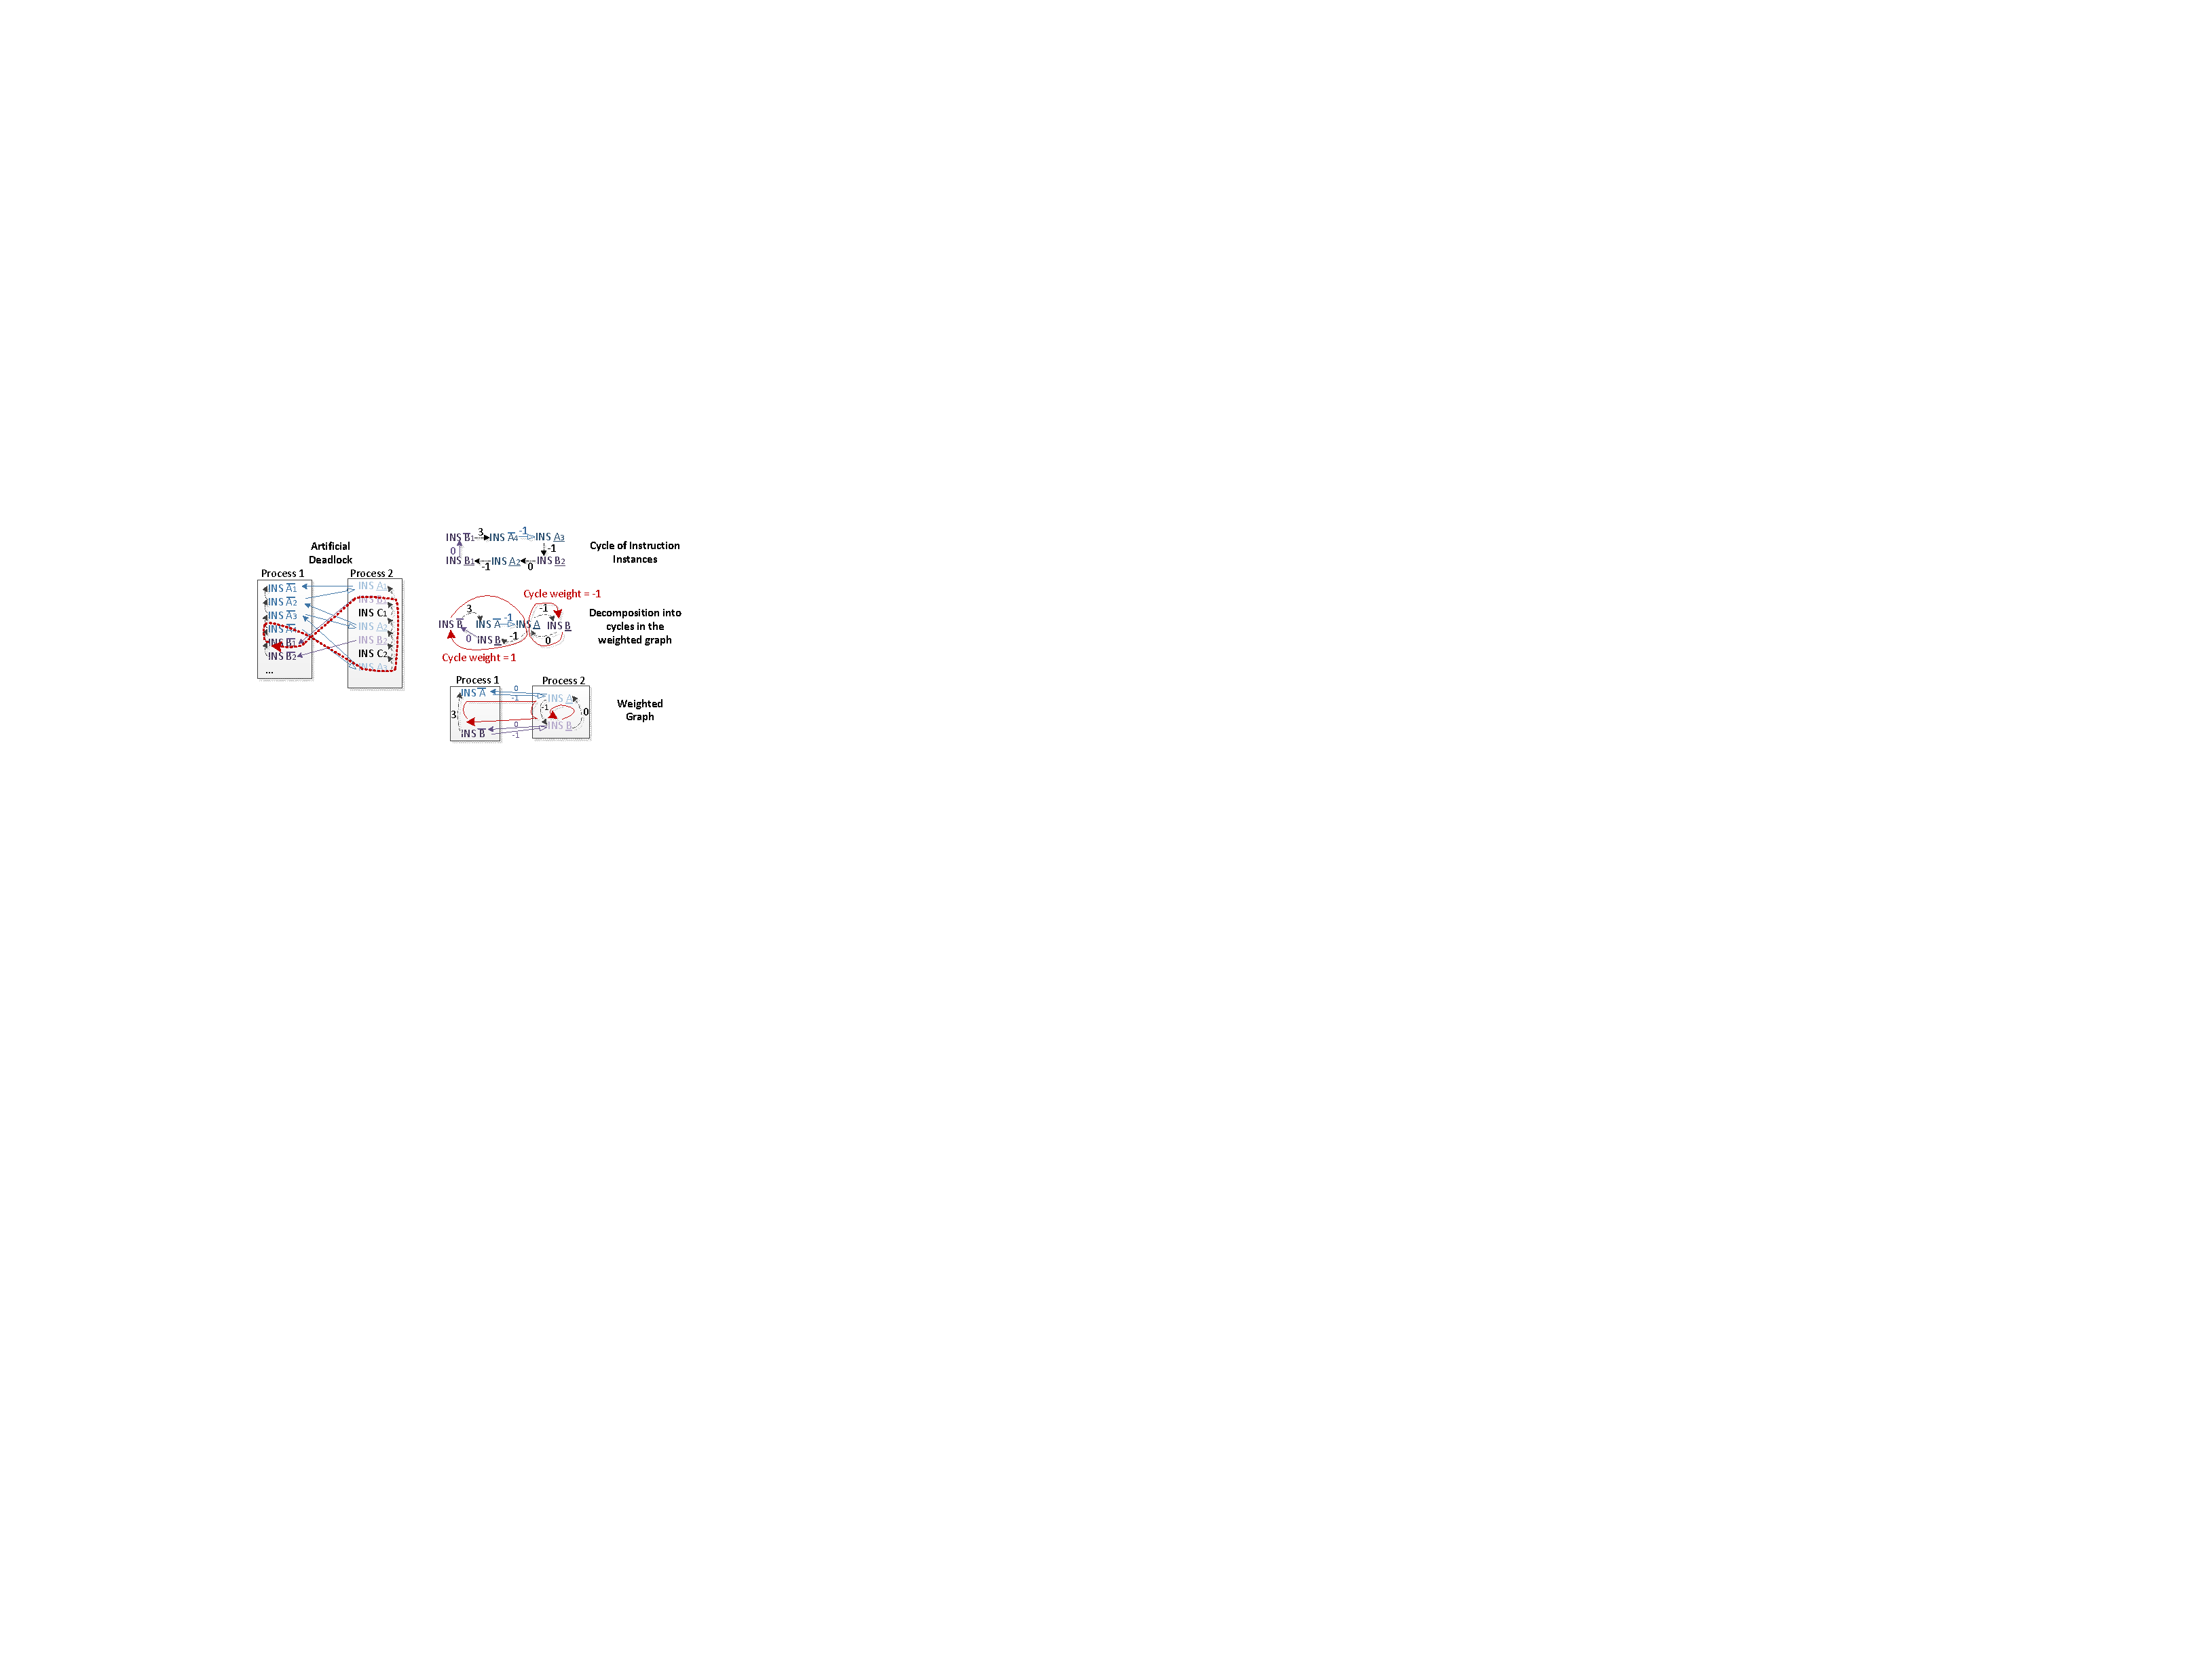
\includegraphics[width=0.9\linewidth]{chap4fig/decomp.pdf}
\caption{Decomposition of Cycle of Instruction Instances 
\label{fig:decomp}}
\end{center}
\end{figure}



As lemma~\ref{deadlock2cycle} is proven to be true, the absence of cycles of
weight $\vec{0}$ or with positive leading elements guarantees the the absence of artificial deadlock (the contrapositive).

\begin{comment}
In addition, the number of $DepS$ edges added can also
be reduced. Only the scheduling of producer/consumer instructions matters for
deadlock detection, therefore any $DepS$ edges having end point $j \not\in \bar{J^p} \cup \underline{J}^p$ can be omitted.For
the experiments we performed in chapter~\ref{decoupleChap}, we extract the
schedule from the HLS report and with FIFO size set to 64, no
potential deadlocks are detected.

With the detection mechanism in place, we can try to resolve the found deadlock by
increasing the FIFO capacity. In the case of using simulations for deadlock detection, there is always one FIFO whose capacity needs to be increased when a deadlock occurs. 
In our approach, however, if multiple $DepF$ edges are present in the cycle,
it's not immediately apparent which FIFO should be modified. There can also be
multiple cycles sharing some of the $DepF$ edges, 

there is a difference from the cases when simulation was used,
it may.  
\end{comment}



\begin{comment}

\begin{figure}[htp]
\begin{center}
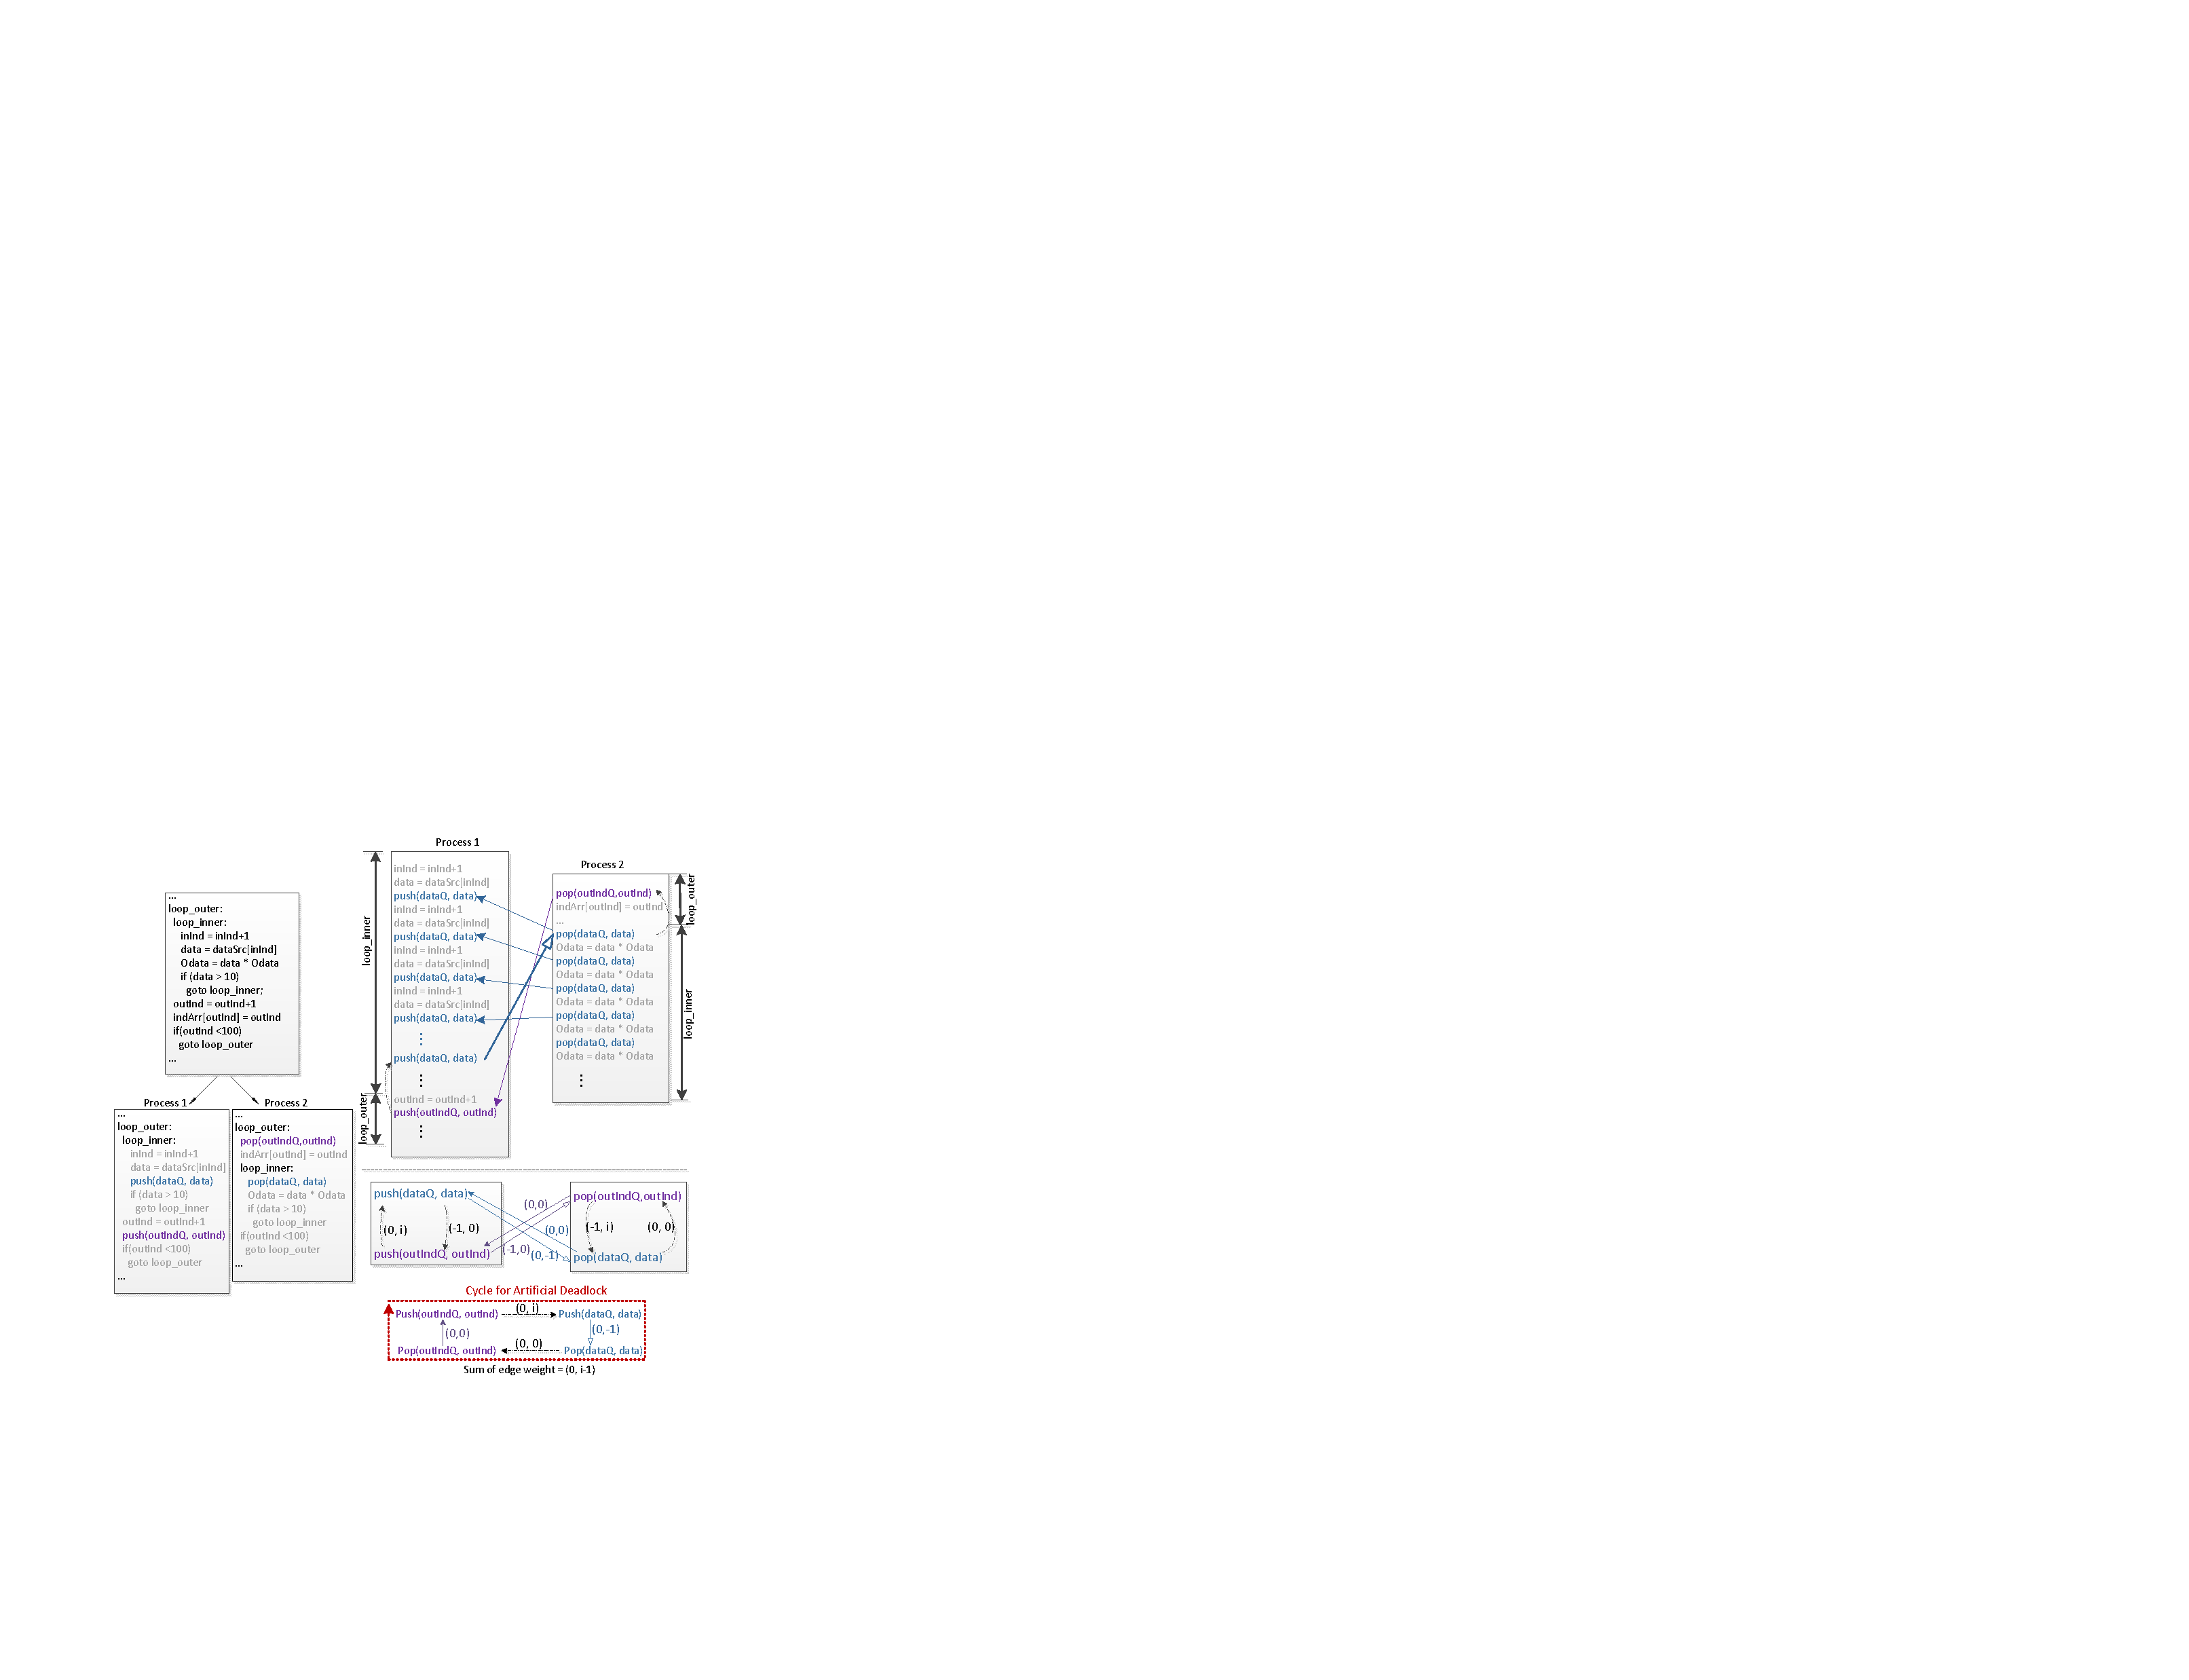
\includegraphics[width=1.1\linewidth]{chap4fig/unresolve.pdf}
\caption{Rescheduling Creates Statically Unresolvable Deadlock
\label{fig:badsitu}}
\end{center}
\end{figure}

\subsection{Statically Unresolvable Artificial Deadlocks}
Using the analysis framework we have formulated, we can construct situations
where artificial deadlocks may always occur, regardless of how much
space is statically assigned to a FIFO channel. Figure~\ref{fig:badsitu}
shows one example where no guarantee of deadlock freedom can be
statically obtained. 
Here, the outer loop consumer instruction
are rescheduled to before the start of the inner loop, while the corresponding producer instruction
executes after the completion of the inner loop iterations. As the
number of iterations of the inner loop is statically unknown, there will
always be a $DepF$ between a pair of the $push$ and $pop$ instruction instances (and therefore a cycle of dependence),
regardless of how large the FIFO size is. 

In the weighted edge graph, the size of the iteration space is represented
symbolically and the $DepS$ edge between the outer loop and inner loop producers carries a weight of $(0,i)$. Assuming FIFOs of size 1, a cycle of weight $(0, i-1)$ is found. Without knowing the bound of $i$, there is no way we can add enough
space to the $DepF$ edge between the producer and consumer of ``data" such
that the cycle weight has negative leading element.


The actual computation is shown
in this example to demonstrate the validity of the reordering. There is no local data dependency violated, yet artificial deadlocks are created in the network.
To prevent this type of unresolvable deadlocks, we can impose constraints on the
reordering of instructions performed by the HLS tools. The starting point of
instruction rescheduling is always the original program order, or more specifically the locally consistent $G(p)$. In the weighted graph representing the network of processes each scheduled according to $G(p)$, $DepS$ edges going from an instruction to its predecessor in the inner most loop all have weight $\vec{0}$. The weight of a $DepS$ edge from an outer loop instruction towards a preceding inner loop instruction has its leading element equals to the max number of inner loop iterations minus 1.
On the other hand,
The $DepS$ edge pointing to successors always has element -1 at 
the position of the vector corresponding to the outermost loop level among
the two instructions. 

In order to avoid creating unresolvable deadlocks,
we shall disallow any reordering creating cycles whose weight has non-statically
known leading elements. This can happen in two ways: 1) a statically unknown symbol
is added to the leading element of a cycle or 2) a new leading element is exposed
because the original one becomes zero. To prevent these scenarios, we can constrain changes at every edge. More specifically, 
rescheduling of instruction with respect to another instruction at the same level in the loop nest has additive effect on the edge weight. The extent
of rescheduling in HLS, however, is in general known statically, so it  



We have already proven that when all processes are scheduled  according to $G(p)$, there will be no artificial deadlocks, let alone unresolvable artificial
deadlocks. This does not mean there can be no cycles with zero 
Any reordering which causes a statically unknown number to become
leading element in any of the cycles can potentially create an unresolvable
artificial deadlock

Therefore, any addition of statically known number to non leading elements of the $DepS$ edges will not result in unresolvable deadlock as well. The sum of cycles can be changed back by adding capacity in one of the $DepF$ edges.
As a result, any instruction reordering in the innermost loop can be 
permitted. 
However, if an edge whose leading element goes from -1 to 0, it may now have a new leading element, which can be a statically unknown value. There is a possibility we now have a cycle weight whose leading element is statically unknown. 
\end{comment}



\begin{comment}
Specifically, the amount
by which an instruction instance is moved ahead of its predecessors in the original program order must be known statically.

It was proven that when each $p \in P$ execute according to the original
problem order, no artificial deadlock would occur even when the FIFOs are of size one.
We have also demonstrated that with certain rescheduling, deadlock freedom
can become unachievable with finite FIFO size. We can thus devise a set of 
constraints for the HLS tools when they are applied in our pipeline generation flow.





Our example shows that when producer (or consumer) instructions are rescheduled with respect to other instructions in their own process, more tokens may
need to be buffered before the consumer instruction is activated. To ensure progress
of the network, we need to size the FIFOs such that a
consumer instruction instance is always scheduled before the cycle of blocked
processes is formed.
\end{comment}


\subsection{Effect of Bursted Memory Accesses}
We have been modeling the memory as a special process who responds to the requests in a FCFS fashion. The use of bursted memory access can sometimes complicate this
assumption.

























\begin{comment}
\subsection{Compute FIFO Sizes for Artificial Deadlock Freedom}



Let the new schedule after instruction reordering for $p$ be $F(p)$, to ensure no artificial deadlock is introduced after intra-process rescheduling,
the minimum FIFO sizes can be determined as follows:
\begin{itemize}
\item If an instruction $j'$ is a consumer instruction, let its ``contribution"
to the size of the FIFO it reads from be $Q$,  $Q$ should satisfy:

\begin{equation}
\label{ineq1}
Q > \max_{y,j''}(x_1-x_2)   
\end{equation}
\begin{gather*}
\text{where $j'_{x1} \prec j''_y$ \text{in} $G(p)$ and
$j''_y \prec j'_{x2}$ \text{in} $F(p)$}
\end{gather*}
%\end{aligned}
%\end{equation}


\item If an instruction $j'$ is a producer instruction,
let its ``contribution"
to the size of the FIFO it writes to be $W$,  $W$ should satisfy:
\begin{equation}
\label{ineq2}
W > \max_{y,j''}(x_2-x_1)   
\end{equation}
\begin{gather*}
\text{where $j''_y \prec j'_{x1} $ \text{in} $G(p)$ and
$j'_{x2} \prec j''_y $ \text{in} $F(p)$}
\end{gather*}

\item To avoid artificial deadlock, for each FIFO in the network, its size $C$ should satisfy:

\begin{equation}
\label{ineq3}
C > Q+W
\end{equation}
\begin{gather*}
\text{$Q$, $W$ : contributions from~\ref{ineq1} and~\ref{ineq2} respectively}
\end{gather*}
%$W > \max_{x,j''}(y_2-y_1)$ where $j'_{x} \succ j''_{y1}$ in $G(p)$ and  $j''_{y2} \succ j'_{x}$ in $F(p)$
\end{itemize}

In the case of~\ref{ineq1}, we look at the instance of $j''$ which succeeds a set ($R'$) of the consumer instruction instances in $G(p)$, but precedes them in $F(p)$. The max
size for $R'$ after we examine every instance of every $j''$ in $p$ would give us
the FIFO size needed to counter the effect of this rescheduling. The intuition is to have enough buffer space such that the corresponding producer of $j'$ can keep generating token until the artificially
moved predecessors in the new schedule are finished.

For~\ref{ineq2}, on the other hand,  we look at the instance of $j''$ which precedes a set ($R''$) of the producer instruction instances in $G(p)$, but succeeds them in $F(p)$. Similar to the first case, the size of the set is reflective
of how much more buffering we need because of the rescheduling of instructions.
Here we are trying to allocate enough space so
$j'$ can keep producing token without being blocked on write, until the artificially created successors
in the new schedule are done.



\begin{lemma}
\label{boundedRescheduled}
If FIFOs are sized according to~\ref{ineq3}, the network of rescheduled
processes is not going to experience artificial deadlock.
\end{lemma}







\begin{lemma}
\label{consistent}
The set of instruction instances from the producer/consumer pair for each FIFO
is always globally consistent with $H$ if
Given (1) blocking write and (2) all FIFOs having a size of one, all possible  

Given (1) blocking write, (2) G(p) $\forall p$ being locally consistent to $H$, and (3) FIFOs all having a size of one, all possible execution of $N$ would have the set $\{i_k^p:
i \in \bar{I^p} \cup \widetilde{I^p}, \forall p, k \in \Bbb{Z}\}$ being globally
consistent to $H$.
\end{lemma}

We can prove lemma ~\ref{consistent} by contradiction. If the set of instruction instances is not globally consistent with $H$, then there
must be a case where  $i_x^{p1}' \prec i_y^{p2}''$ in $H$, yet  $i_y^{p2}'' \prec  i_x^{p1}',  \exists H_e $. 

\begin{addmargin}[3em]{2em}
From condition (2), we know that $p1 \neq p2$, 
otherwise $G(p1) = G(p2)$ is not locally consistent.  



\end{addmargin}

Due to the fact that $i_y^{p2}'',i_x^{p1}' \in \bar{I^p} \cup \widetilde{I^p}$

The generated $H$ is apparently an interleaving of a set of consistent $G(p)$  $\forall p\in P$. From the FIFO channels' perspective, as long as the relative ordering of producer instruction instances $\bar{i_k}(p)$ and the consumer placeholder instruction instances $\widetilde{i_k}(p')$ is consistent with $H$,
the maximum number of tokens possible in each channel would be one. That is,
if  $\bar{i}_{k+1}(p)$ is always executed after all the $\widetilde{i_k}(p')$,
there will be no need for more than one slot in each FIFO channel.



Knowing that for any 

If we allow each process to run in a data driven manner~\cite{}, where the
availability of data in an input port 




Realize however, the
network generated from a sequential program however, is a special
case amongst all the KPNs. We claim that the  
\end{comment}



%\newpage
%\section{Deadlock-Freedom in Elastic Computational Pipeline}
